\section*{Aufgabe 3}

\subsection*{a)}
$ d_{ik} = (log(f_{ik} +1 ) * log (\frac{N}{n_{k}}) $\\

\begin{tabular}{|c|c|c|c|c|c|}
 & $D_{1}$ & $D_{2}$ & $n_{k}$ & \multicolumn{2}{c}{$d_{ik}$} \\ 
\hline 
 & $D_{1}$ & $D_{2}$ & $n_{k}$ & $D_{1}$ & $D_{2}$ \\ 
\hline 
the & 0 & 3 & 3 &  \\ 
\hline 
two & 0 & 1 & 1 &  \\ 
\hline 
manning & 1 & 1 & 2 &  \\ 
\hline 
brothers & 1 & 2 & 3 &  \\ 
\hline 
are & 1 & 1 & 2 & \\ 
\hline 
only & 0 & 1 & 1 &  \\ 
\hline 
quarterback & 1 & 1 & 2 &  \\ 
\hline 
who & 0 & 1 & 1 &  \\ 
\hline 
won & 0 & 1 & 1 &  \\ 
\hline 
super & 0 & 1 & 1 &  \\ 
\hline 
bowl & 0 & 1 & 1 &  \\ 
\hline 
peyton & 1 & 0 & 1 &  \\ 
\hline 
and & 1 & 0 & 1 &  \\ 
\hline 
eli & 1 & 0 & 1 &  \\ 
\hline 
\end{tabular} 
\subsection*{b)}
Die wesentliche Idee des TW-IDF Modells ist es Termgewichte zu verwenden. Dazu wird zuerst ein Graph eines Textes erstellt. Danach werden die Eingangsgrade der unterschiedlichen Knoten berechnet. Mit diesen Eingangsgraden wird dann ähnlich wie bei der TF-IDF ein Score berechnet. Im TF-IDF-Modell hingegen werden dazu nicht die Termgewichte sondern Termhäufigkeiten verwendet.
\begin{figure}[H]
\centering
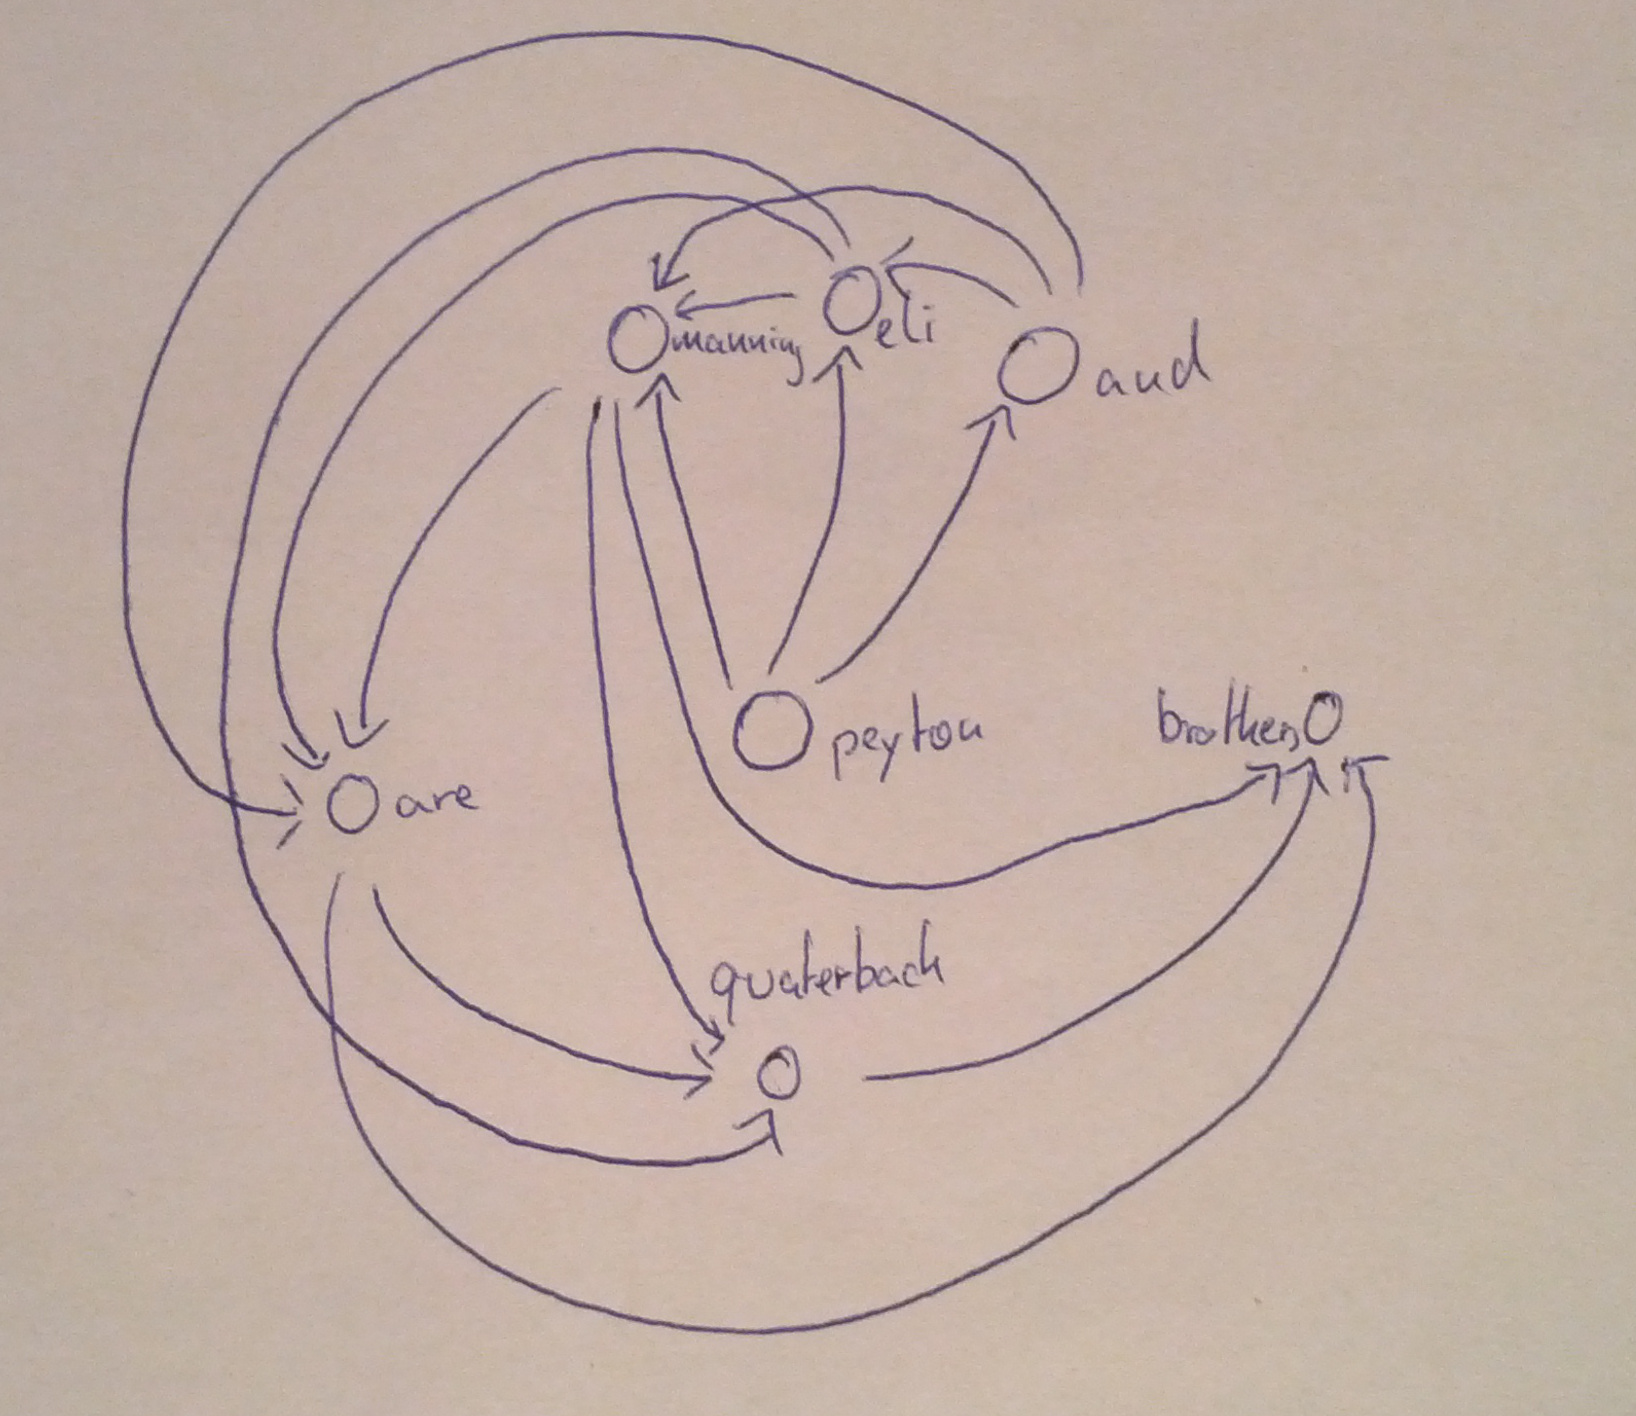
\includegraphics[width=0.7\linewidth]{./Aufgabe3/Graph.jpg}
\caption{Graph für $D_{1}$}
\label{fig:Graph}
\end{figure}

\subsection*{c)}

\subsection*{d)}
\subsubsection*{i)}
Die Autoren begannen mit nicht-gerichteten Kanten um ein Auftauchen von zwei Termen zu berücksichtigen unabhängig von ihrer Reihenfolge. Im weiteren Verlauf verwendeten sie dennoch gerichtete Kanten um natürlichen Fluss eines Textes zu umfassen und führte in der Praxis auch zu statistisch signifikant besseren Ergebnissen, die sich aber in den Kennzahlen MAP und P@10 nur kaum äußerten.
\subsubsection*{ii)}
Die Autoren entschieden sich, obwohl es an manchen Stellen sinnvoll erscheint gewichtete Kanten zu verwenden dagegen, da in der Praxis die Verwendung von ungewichteten Kanten einheitlich zu besseren Ergebnissen führt.
\subsubsection*{iii)}
Die Autoren legten bei ihrer Arbeit die Fenstergröße auf 4 fest, da sie keine signifikant besseren Ergebnisse bei einem zwischen 6 und 30 (wie von Blanco und Lioma verwendet) variierenden Wert beobachten konnten. Der Wert wurde auf 4 festgesetzt, da die Autoren (im Gegensatz zu Blanco und Lioma) sogenannte \glqq Stoppwörter\grqq im Vorlauf entfernten. Der kleine Wert wurde auch aufgrund der Berechnungskosten gewählt (die sich linear zur Fenstergröße verhalten)
\subsection*{e)}
Abbildung 3 zeigt einen Vergleich unterschiedlicher Retrieval Modelle die auf WT10G angewendet wurden.\\
Dabei wird dargestellt, dass z.B. das Modell TW-IDF ohne Normalisierung (b=0) sehr hohe Relevanz-Werte bei längeren Dokumenten erzielt, aber dahingegen relativ niedrige Relevanz-Werte bei kürzeren Dokumenten. Wohingegen das Modell TW-IDF mit Normalisierung (blaue Linie mit Dreiecken) schon sehr gut mit der Wahrscheinlichkeit der Relevanz (graue Linie mit Kreisen) deckt.\\
Das Vektor-Raum-Modell TF-IDF erzielt insgesamt zwar konstante aber im Vergleich zur Relevanz bei kürzeren Dokumenten sehr hohe Relevanz-Werte und bei längeren sehr niedrige.\\
Das Wahrscheinlichkeitsmodell BM25 schneidet zwar erheblich besser ab, wird aber dennoch vom TW-IDF mit Normalisierung \glqq geschlagen\grqq . Die Autoren begründen das mit der Nutzung von Termgewichten statt Termhäufigkeiten.